%profilingresults


Figure \ref{fig:dfsa} shows the profiling results for the throughput (update rate) of the Vanishing Point algorithm for different CPU-GPU allocations of the 3 tasks and different frequencies of the CPU and the GPU. 
Note, the CPU can be clocked upto 2.32 GHz (on all 4 cores), while the GPU can be clocked upto 0.852 GHz. 
We select 6 operating frequencies evenly spaced from the minimum and maximum Jetson CPU and GPU frequencies for both the CPU and the GPU. 
In these figures, the 3 letter combinations encode the CPU-GPU allocation .
For example, C G C means that the Blur was run on the CPU, Canny on the GPU and the Hough transform on the CPU.


\begin{figure}[htbp]
	\centering
	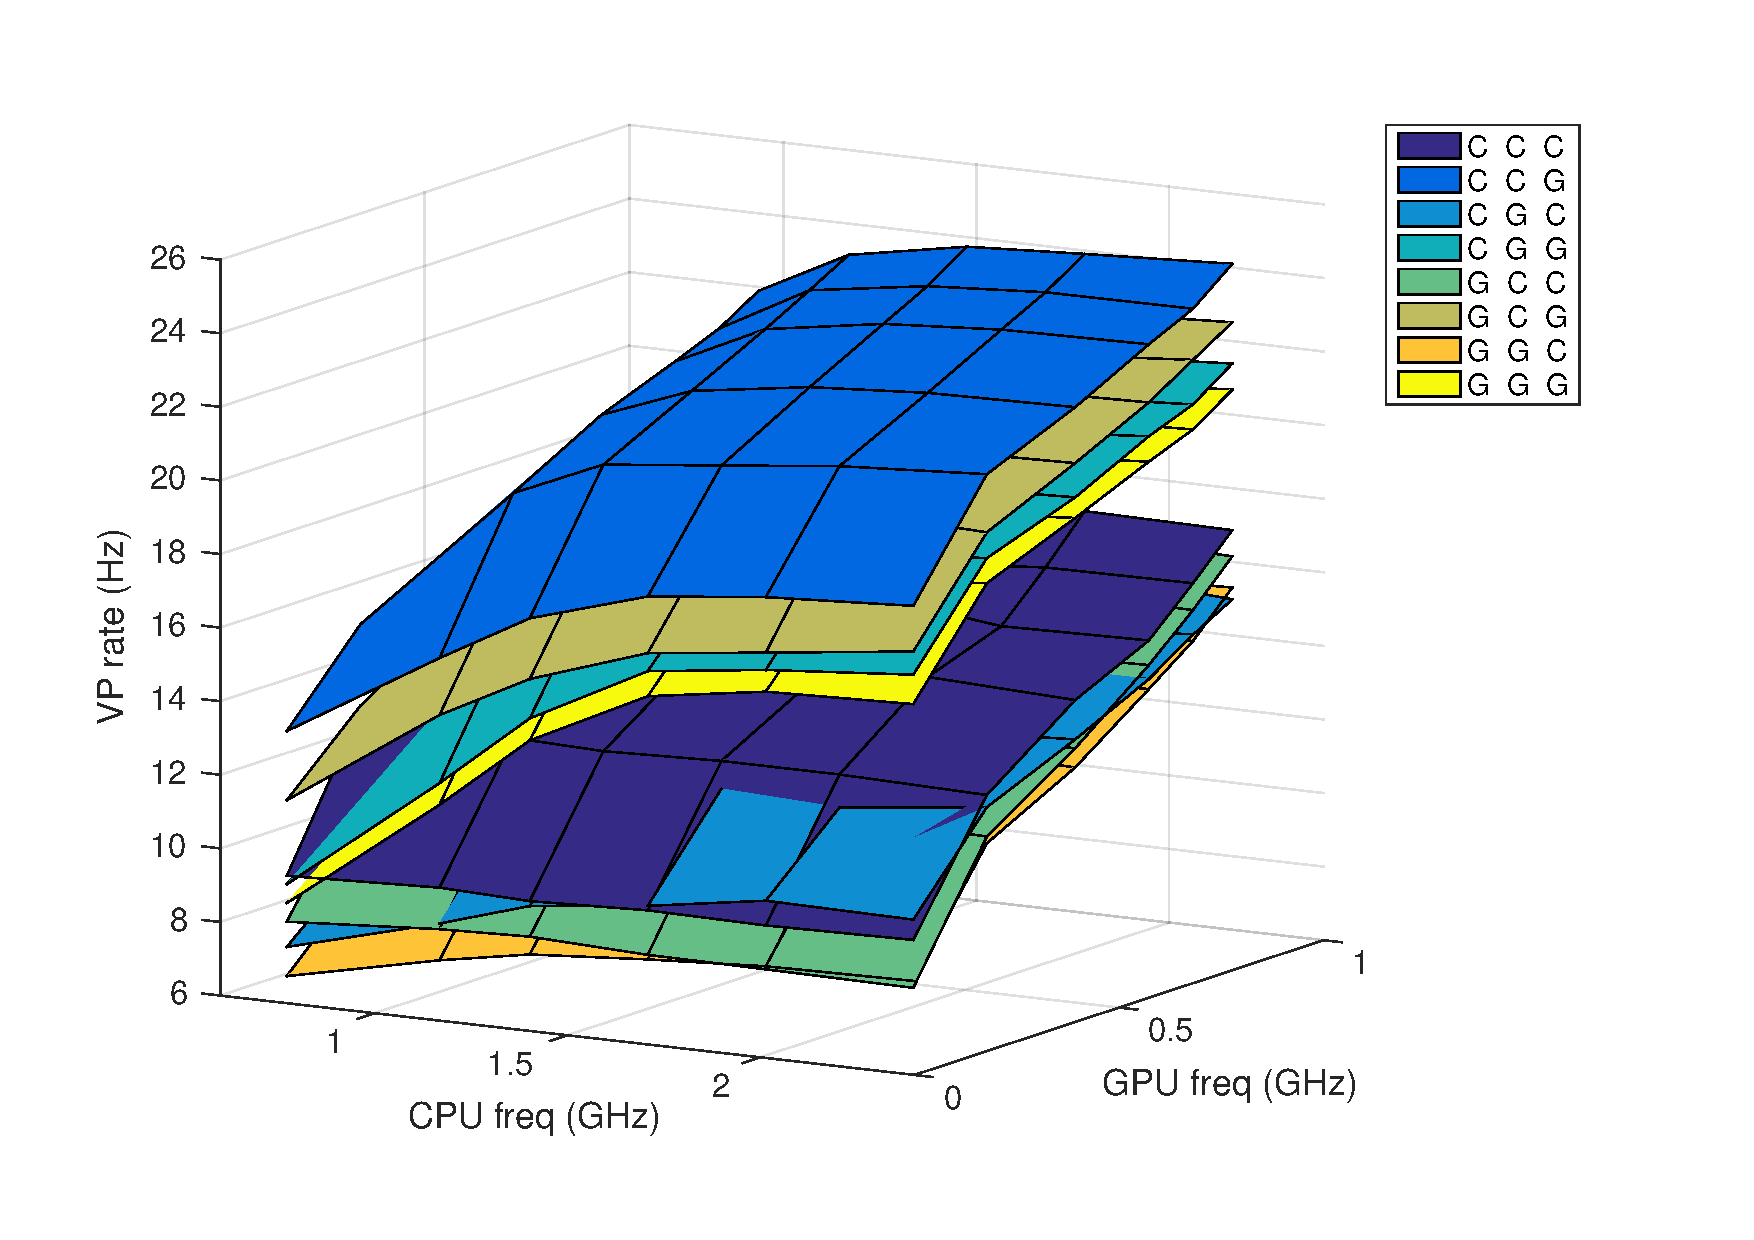
\includegraphics[width=0.46\textwidth]{Figs/surf_Rate.pdf}
	\caption{Vanishing point algorithm update rate for different CPU-GPU assignments at varying frequencies (color in online version).}
	\label{fig:sfda}%same freq diff assignment}
\end{figure}

%\begin{figure}[hbtp]
%\centering
%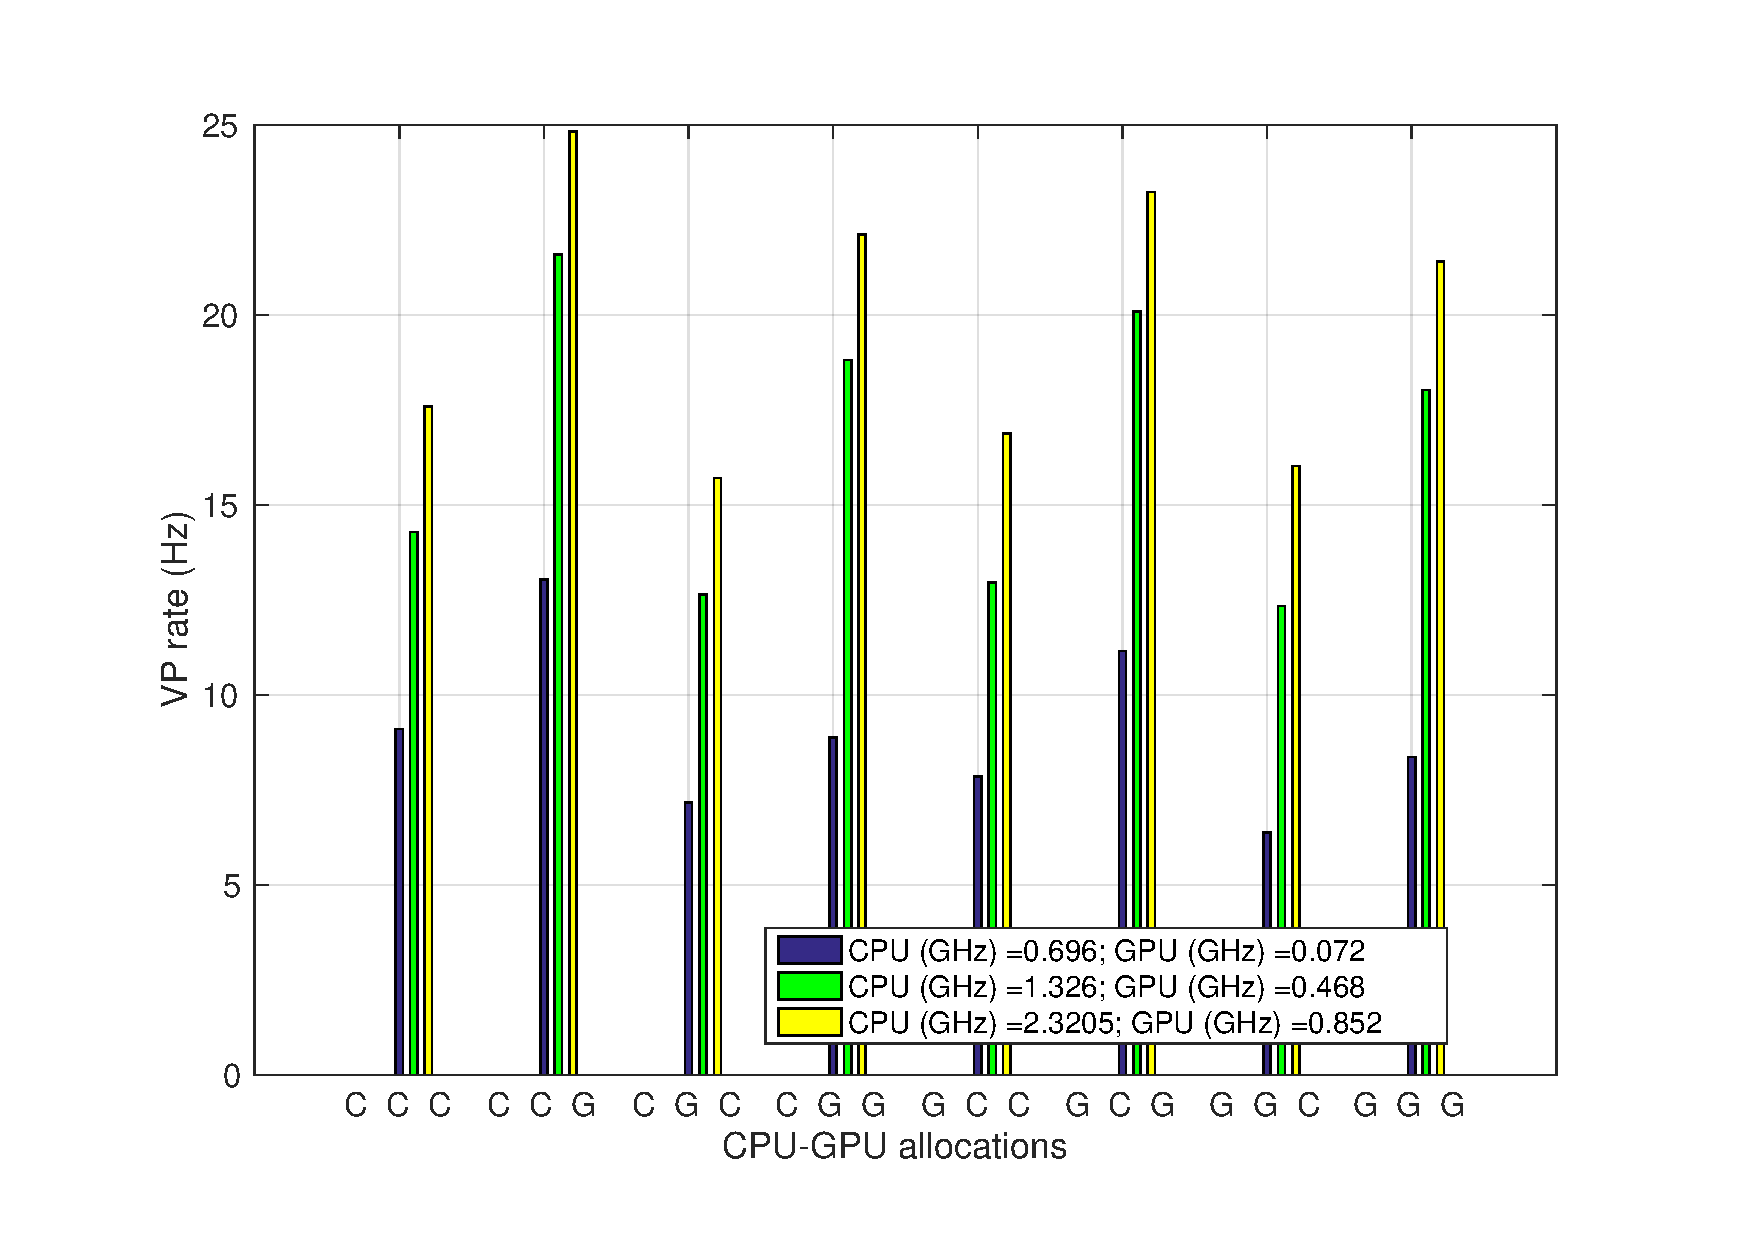
\includegraphics[scale=0.3]{Figs/RateHist.pdf}
%\caption{Control update rate for different frequencies and a given CPU-GPU assignment. For clarity we only consider 3 CPU and GPU frequencies for this %figure, ranging from the minimum to the maximum of frequencies of CPU and GPU. (Color in online version) }
%\label{fig:dfsa} %diff freq same assignment}
%\end{figure}

Figure \ref{fig:sfda_pow} showS the profiling of average power consumed during the computations for the vanishing point over all frames in the video used for the profiling.


\begin{figure}[htbp]
	\centering
	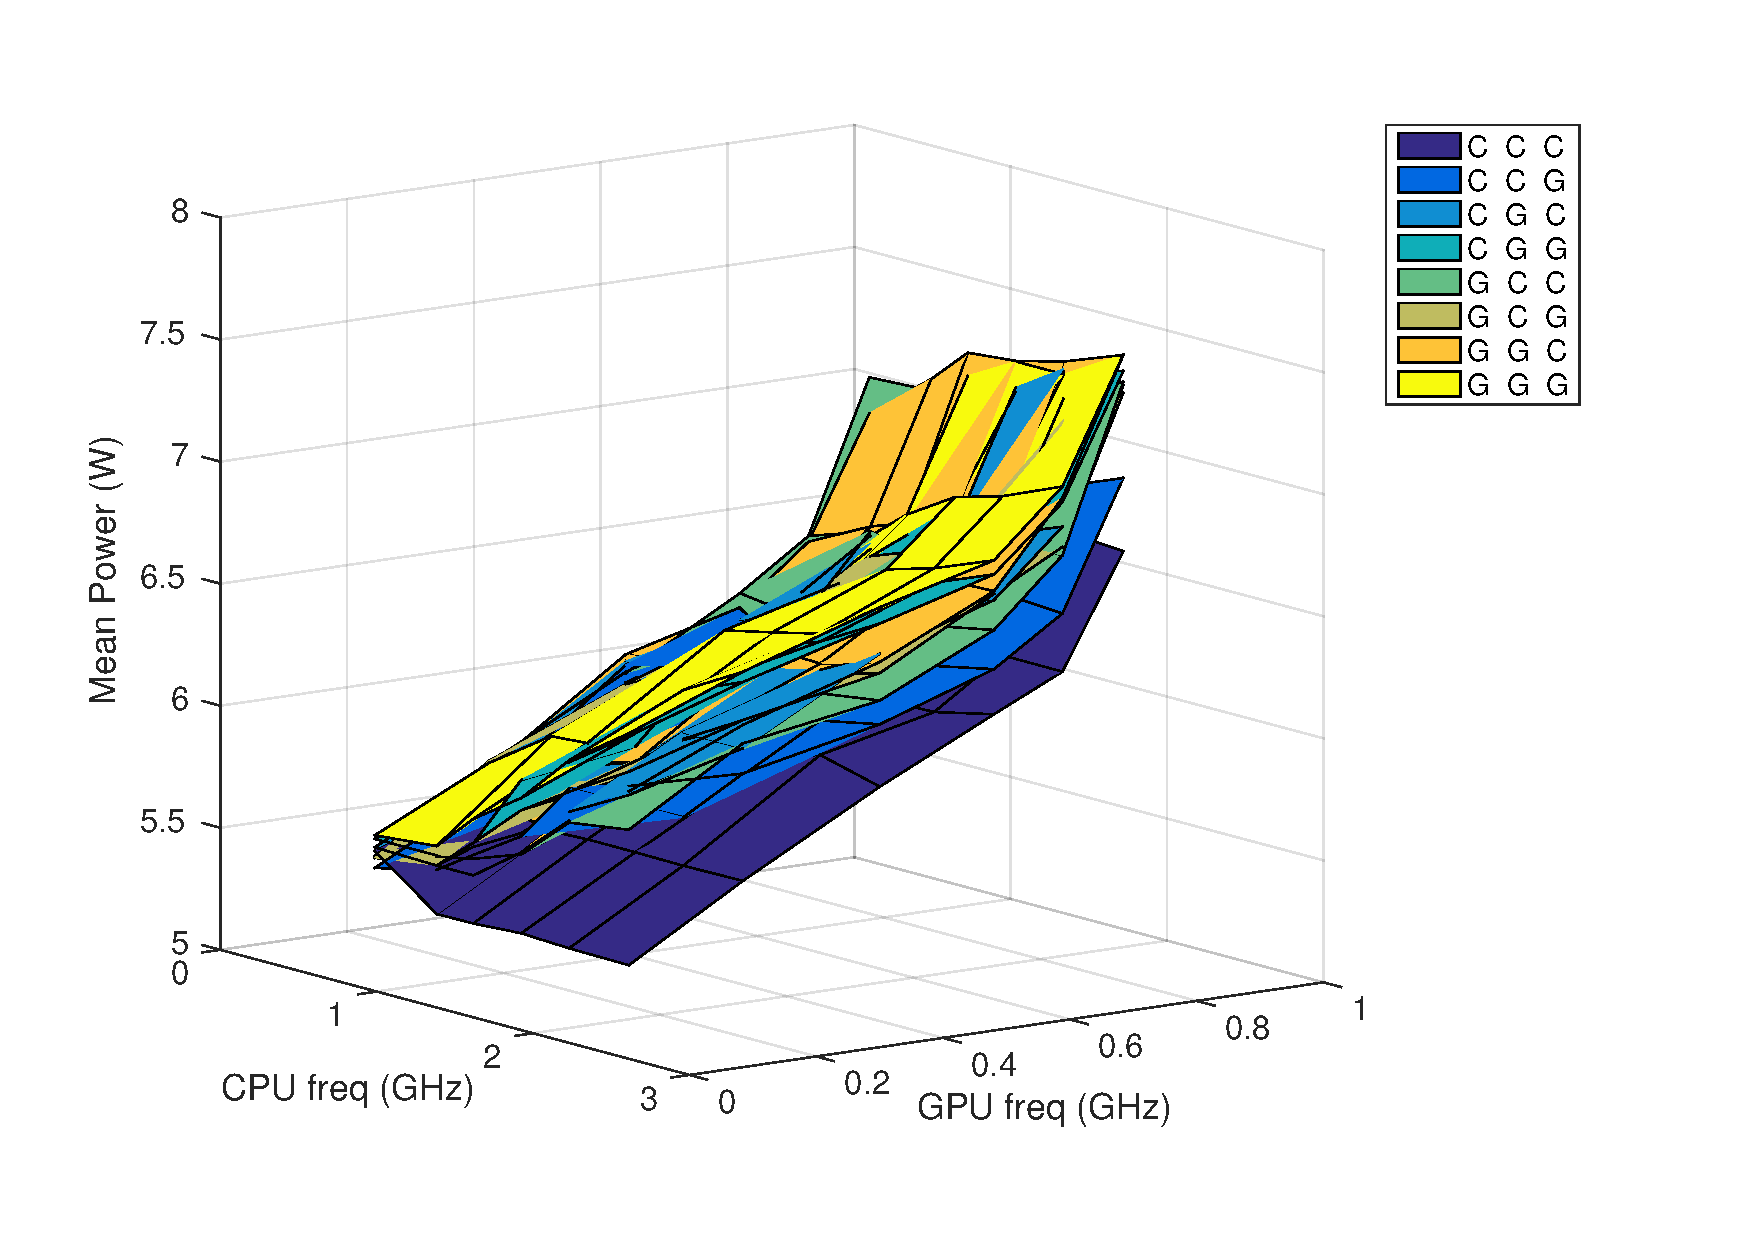
\includegraphics[width=0.46\textwidth]{Figs/surf_Power.pdf}
	\caption{Mean power consumed by the Jetson for different CPU-GPU assignments at varying frequencies. (Color in online version)}
	\label{fig:sfda_pow}%same freq diff assignment}
\end{figure}

%\begin{figure}[htbp]
%\centering
%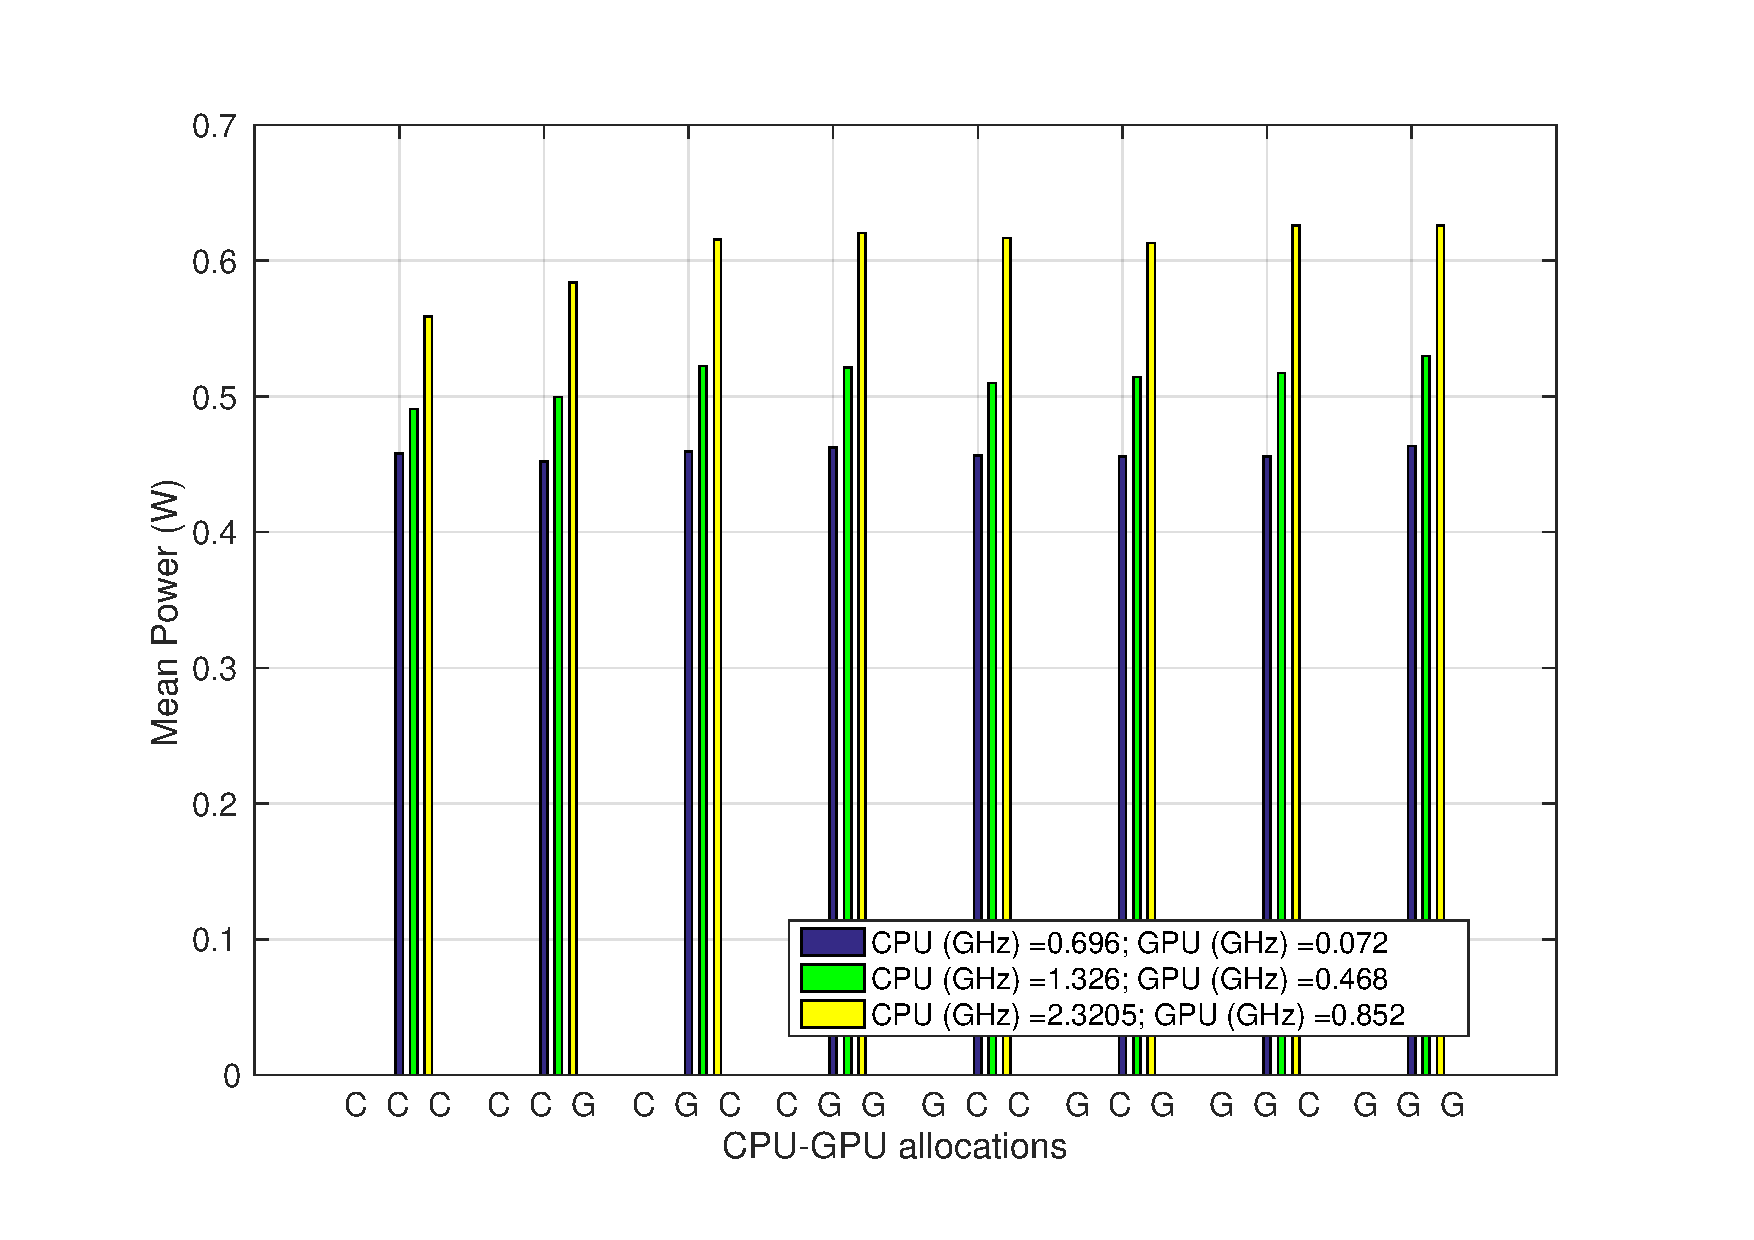
\includegraphics[width=0.46\textwidth]{Figs/PowerHist.pdf}
%\caption{Mean power consumed by the Jetson for different frequencies and a given CPU-GPU assignment.  For clarity we only consider 3 CPU and GPU frequencies for this figure, ranging from the minimum and maximum of both the CPU and the GPU. (Color in online version)}
%\label{fig:dfsa_pow} %diff freq same assignment}
%\end{figure}